\section{Introduction}\label{section:Introduction}
Many permission models today are broken for the type of applications being used today. We've gone from systems that run only trusted programs to PCs, mobile devices, and other systems where users want to run untrusted or semi-trusted code. The permission models have not kept pace with the change in computing landscape. Existing permission models either protect only from other users, ignoring the threat of untrusted code, provide shallow and overly broad protections, or use unwieldy and complicated configuration mechanics. We present a new permission model based on the idea that you have data to protect, and you want to protect it against snooping applications. We design and implement our language inside of Racket\cite{racket}. We evaluate our base implementation by building up two common command line programs, ls and cat. Using these programs we evaluate our permission model to prevent access to certain resources.

\section{Related Work}\label{section:relatedwork}
Related work includes the Unix permission model, mandatory access control systems, and the Android permission model.

Unix permissions provide a simple and useful model for protecting against other users on a system, but they do not protect a user against malicious applications.

Mandatory access systems give greater protections, and are generally extensions of the Unix model that work with it.  These include SELinux, AppArmor, Tomoyo Linux, Capsicum, and Tame.
SELinux\cite{selinux} is used both on Android and Linux to constrain applications from accessing or using Kernel nodes, directories, files or sockets.
AppArmor and Tomoyo are additional optional systems for Linux which restrict applications based on configurable application contexts.
FreeBSD has Capsicum\cite{capsicum}, a capability based system which essentially sandboxes applications. 
OpenBSD has a new mechanism \textit{tame()}\cite{tame} which is a subsystem  to restrict programs into a "reduced feature operating model".
All of these mandatory access systems have complex models that are difficult for users to understand.  
They must be configured with complicated text files that can be edited only by root.  
This makes it impossible for normal users to control them, or for non-root users to set their personal security policy.

Android re-purposes the classic Unix permission model by treating each application as a different user, and has a variety of different high-level permissions that applications can request.
The Android security model is the most commonly used model on consumer devices, and some consider it to be the state of the art.
However, the Android permission model has many flaws.
Permissions must be granted at install-time, which most users don't pay attention to.
Many permissions are overly broad, such as full sd-card access.
Many permissions have confusing names and descriptions, and it is difficult to find out what they really do.
All permissions must be granted, so users can not allow partial access to applications to get the functionality they desire while blocking functionality they want to disallow.
Finally, all permissions are designed by Google, whom many view as an adversary, with no possibility for extension by other parties that the user trusts.
Android version 6 was released while we were working on this project, which allows run-time permission configuration, fixing some of the issues, but the others still exist.

\section{Adversary Model}\label{section:adversary-model}
Our adversary model is based around the creators of the software that you install on your device and what information can be gathered/changed without your knowledge. We classified our adversary's into two main categories, Legitimate Advertising Businesses and Malware Distributors.

Legitimate Businesses typically provide the software free of charge but gather personal information available on your device to be used for advertising purposes.  While they are legal entities they are often viewed as malicious, or at least overstepping their bounds on data collection, and tend to scoop up much more personal information than people realize or want to allow. Typical examples of these entities are Google and Facebook.  

Malware Distributors also provide software that appears to have a legitimate purpose. The legitimate purpose is used to mask the true malicious nature of the software. The goal of these adversaries is typically unlawful activities that can cause the user harm. This can be destruction of data, ransomware, identity theft and botnet creation. Typical examples of these type of adversaries are Crypto-Locker, Spam Distributors, and people on Darkode.

These code written by these adversaries is knowingly run by users, although they do not know what the software does.  Adversaries generally have access to file system and network resources on the user's device, and are only limited by access and permission systems used by the operating system or runtime environment.

\section{Methodology}\label{section:methodology}
We have created a model that includes primitive permissions that take arguments, a means of combination for these primitives, and a novel method for protecting sensitive resources.
Since all user data is stored on the file system, and devices and other resources on Unix are accessed as files, security of the file system is the core of our model.
We use s-expression notation to write down our permissions, and the most basic permission in our system is \textit{(fs-read "/file/system/path")}.  
The \textit{fs-read} permission allows an application to read the file or directory at the path given in its argument, as well recursively to any sub directories and their contained files.
The \textit{fs-write} permission similarly grants write permission.
It is often convenient and desirable for users to give read or write permissions to applications at the root of a large sub-tree, such as a user's home directory.  
However, there are often some sub-directories in that tree that are more sensitive, such as directories containing passwords, private keys, or sensitive data.
To allow the convenience of recursive access to large parts of the file system tree while still providing protection to sensitive sub-trees, we provide the \textit{fs-protect} pseudo-permission.
\textit{fs-protect} puts a protective barrier on its given path, blocking access to all sub-trees of that path without an \textit{fs-read} or \textit{fs-write} permission with an argument explicitly allowing that sub-tree.

For example, if a user has \textit{(fs-protext "~/.ssh")} in his global permission configuration, and \textit{(fs-read "~")} in his configuration for the \textit{foo} application, \textit{foo} can access \textit{~/Documents/paper.odf} or \textit{~/text-messages/personal-conversation-history.dat}, but not \textit{~/.ssh/id\_rsa} or \textit{~/.ssh/known\_hosts}.  
If the \textit{bar} application has \textit{(fs-read "~/.ssh/known\_hosts")}, it can access \textit{~/.ssh/known\_hosts} (and any sub directories of it if it were a directory), but not \textit{~/.ssh/id\_rsa}.
This allows for both convenient broad access permissions as well as very fine-grained access.

In addition to primitive permissions, composite permissions can be created as functions from higher-level permissions to primitives or other composite permissions.  This allows for abstraction to form high-level permissions such as those seen in Android.  For instance, if calendar files are stored in \textit{~/app-data/calendar/}, then permissions to a user's work calendar may be given by adding a \textit{(calendar "work")} permission that expands into \textit{(fs-read "~/app-data/calendar/work/")} and \textit{(fs-write "~/app-data/calendar/work/")}.  This makes it easy to add many high level permissions, while also providing an easy way for users to see the expansion of such permissions to know what they really do.  New composite permissions must be defined as simple pattern-matching replacements, so that both their abstract and specific expansions can be displayed to users easily.

To be useful to both normal and sophisticated users, configuration must be simultaneously easy and powerful, and allow for both graphical editing for normal users and text configuration that can be version controlled for administrators.
To this end we have designed our permissions to be writable as s-expressions, which are easy for programs to read and write, and eminently human-readable and editable.
Our model allows for applications to ask for privileges at run-time, and additionally for them to be disallowed to by configuration.  This also gives the flexibility for our model to be used by different user bases with different requirements.

\section{Implementation}\label{section:implementation}
We created a proof-of-concept implementation of our framework as a language and runtime system built using Racket's hash lang feature \cite{rakt}. Programs written in \textit{permission-lang}, as we call it, have their permissions loaded by the run-time system for checking.
A global permission file is consulted for all applications, as well as an app-specific file.  
When an application uses a file access function, such as \textit{open-input-file} or \textit{write-to-file}, the loaded permissions are checked.  
If permission has been granted, the program continues as normal.  
If permission has not been granted, a dialog box will appear.  
The dialog will show which permission the application is lacking, and present the user with options to allow or deny the permission for the extent of the program run, to permanently allow the permission, or to stop the application from asking for any more permissions.
If the user allows access, the run-time system adds the permission to the run-time permission list and/or to the permanent application-specific permission file.
If the user denies the permission, or if the application is blocked from asking for permission, then access is blocked and an exception is raised.
\\
\indent
Composite permissions are implemented as files in a specific directory with the same name as the permission they give, and containing their pattern and template.  When programs start, these templates are used to expand given composite permissions to primitives.  When an application requests composite permissions from the user, the user can press a button on the dialog to see a one-level expansion of the specific permission.  If the expansion contains composite permissions, the user can expand them as well.  This can be continued until the user sees the permission entirely in terms of primitives.
\\
\indent
We created test programs in \textit{permission-lang}, including an implementations of cat, ls, and a toy calendar program.
These were used to test that permissions were checked and enforced properly, and to test the effectiveness of the user interface.\\
Our implementation is hosted on Github, and you can view our code here \url{https://github.com/ScottyBauer/CS6940-Project}


\section{Results}\label{section:ResImp}
\begin{figure}
\centering
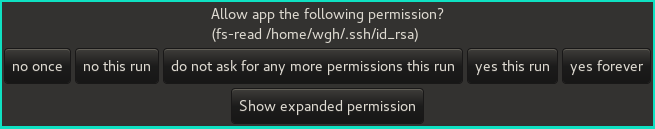
\includegraphics[height=1.5in, width=4in]{ask-permission.png}
\caption{Runtime permission delegation to user}
\end{figure}

\indent
As a proof of concept, we wrapped common Racket file system functions in our language runtime. That means when a program written in our language invokes a file system function, it goes to our runtime which validates that the calling process has the ability to access that function and the parameters for that function. Lets say an application wants to read some specific file. The runtime will look at the file system path to be read and compare the paths against the permission file. If the user had previously granted access to this file then the runtime invokes the true read function and passes the result back the the process. Assuming that the permission had not been granted, the runtime will return an exception to the process.
\\
\indent
To test out or runtime and permission model we built two common unix applications, \textit{cat} and \textit{ls} and ran them using our runtime and permission scheme. We setup a series of directories and files with varying permissions. We attempted to `ls' directories we weren't granted permissions to and verified the runtime stopped us. We also attempted to read files with `cat' we didn't have access to, but did have access to the underlying folder. For all of our tests the permission model and runtime acted as expected. When a user hadn't predefined a set of permissions to use the runtime will pop up a dialog window which allows the user to see what permission is required to access the resource. The user has the ability to grant access or not grant access to the resource. More over, the user can grant access once, grant access for ever, and the same for the inverse, deny once or deny for ever. An example of the popup can be see in Figure 1.


\section{Future Work}\label{section:futurework}

\begin{figure}[h]
\centering
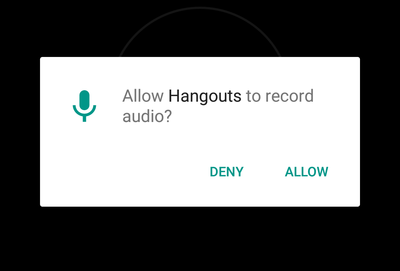
\includegraphics[height=2in, width=2.5in]{app.png}
\caption{Android 6.0 runtime permission check}
\end{figure}

We believe that our work is a step in the right direction and a good iteration on top of some of the previous permission models being shipped today. 
For permission models to be successful they need to be built on a simple set of understandable primitives, and allow useful abstraction on top of them.
They also need to be adaptable to the needs of different users, with both different abilities and different security needs.
Without these attributes, permission systems will be ineffective and inflexible, not providing needed security to most users.
\\
Runtime checking of permissions, as well as the ability to add or revoke permissions at runtime will are an extremely important feature that we built. We argue that this ability to modify permissions at runtime is one of the most important features for a permission system. For example, if a user is near their data cap on their phone, they may wish to revoke permission to use the internet from applications. We believe that the benefits of this feature of a permission model out weighs the burden put on developers who are then required to gracefully handle not having specific permissions at runtime. Android 6.0 has taken this approach\cite{android}, you can now, as a user, revoke certain permissions at runtime. See Figure 2 for an example.\\

We also believe that permission models need to be extensible.
Legacy permission systems such as Android's don't let the user or third parties make new permissions. 
Google creates the permissions and sets what those permissions can and cannot do. 
This isn't in the user's best interest for two reasons. 
First, Google is an advertising company, creating a conflict of interest since they are also viewed as an adversary, and they want to maximize data collection.  
Second, a single company is not able to anticipate the needs of all different types of users.  While the broad permission types defined for Android may work well for many users, others require more fine grained controls.
Permissions systems need to allow for needed fine grained controls and extensibility, while also being easy for the average user to understand and use.
We believe extensible systems built on a simple core are the best way to achieve this, and we therefore recommend further research into such permission models.
\\
\indent
An important improvement our model needs is a set of primitives for networking.  We believe that networking, as well as ony other type of permissions will also benefit from a simple, understandable set of primitives and a means of composition and abstraction.  We believe appropriate network primitives may include permissions such as \textit{(network "domain.example.com")}.

Another concern we have not solved is about additional supporting infrastructure.  For instance, we believe that packaging and installation-time rules and interfaces for adding compound permission definitions would help prevent confusion, accidental or intentional.

We would also be interested in a study of how easily both normal and expert users learn and understand the principles of our permission model and others, and how effectively they can use them.  
We would like to know how effectively different systems are used by different demographics, both by solo experimentation and also with instruction.



\section{Conclusion}\label{section:conclusion}
\textit{permission-lang} is effective at enforcing permissions while allowing easy configuration.  We found the model of permissions with arguments to be effective at providing granularity, and \textit{fs-protect} allowed an effective way to allow convenient access to large file system sub-trees while still giving required protections.
We believe that composition based on primitive permissions is the most effective way to build a complex permission system, but we believe that confusions could arise from similarly-named permissions or from adversaries spoofing legitimate permission definitions.  This is mitigated by the ability for users to see the expansion of composite permissions, but we believe extra support around the packaging and installation of composite permission definitions should be added.

Our implementation is limited by being in a single language implementation, and it can therefore be defeated by simply writing programs in another language.  So while our implementation serves as a useful proof of concept, to be effective it would need to be implemented at an operating system level.  Alternatively, systems could allow only programs written in \textit{permission-lang}, but such action would be severely limiting and frustrating, similar to other systems which have only allowed one programming language, and we discourage such action.  

Additionally, more primitive permissions are needed.  For instance, network permissions are essential, but missing from our prototype.




